%%%%%%%%%%%%%%%%%%%%%%%%%%%%%%%%%%%%%%%%%%%%%%%%%%%%%%%%%%%%%%%%%%
%%%%%%%% ICML 2014 EXAMPLE LATEX SUBMISSION FILE %%%%%%%%%%%%%%%%%
%%%%%%%%%%%%%%%%%%%%%%%%%%%%%%%%%%%%%%%%%%%%%%%%%%%%%%%%%%%%%%%%%%

% Use the following line _only_ if you're still using LaTeX 2.09.
%\documentstyle[icml2014,epsf,natbib]{article}
% If you rely on Latex2e packages, like most moden people use this:
\documentclass{article}

% use Times
\usepackage{times}
% For figures
\usepackage{graphicx} % more modern
%\usepackage{epsfig} % less modern
\usepackage{subfigure} 

% For citations
\usepackage{natbib}

% For algorithms
\usepackage{algorithm}
\usepackage{algorithmic}

% As of 2011, we use the hyperref package to produce hyperlinks in the
% resulting PDF.  If this breaks your system, please commend out the
% following usepackage line and replace \usepackage{icml2014} with
% \usepackage[nohyperref]{icml2014} above.
\usepackage{hyperref}

% Packages hyperref and algorithmic misbehave sometimes.  We can fix
% this with the following command.
\newcommand{\theHalgorithm}{\arabic{algorithm}}

% Employ the following version of the ``usepackage'' statement for
% submitting the draft version of the paper for review.  This will set
% the note in the first column to ``Under review.  Do not distribute.''
\usepackage[accepted]{icml2014} 
% Employ this version of the ``usepackage'' statement after the paper has
% been accepted, when creating the final version.  This will set the
% note in the first column to ``Proceedings of the...''
%\usepackage[accepted]{icml2014}


% The \icmltitle you define below is probably too long as a header.
% Therefore, a short form for the running title is supplied here:
\icmltitlerunning{An Implementation of Video Sementaition and Classifcation}

\begin{document} 

\twocolumn[
\icmltitle{An Implementation of Video Sementaition and Classifcation\\ based on Video Features Extraction and Machine Learning}

\icmlauthor{Jiaming Song}{jiaming.tsong@gmail.com}
\icmladdress{Computer Science and Technology Department, Tsinghua University}
\icmlauthor{Gerald Yankai Zhang}{zyk12@mails.tsinghua.edu.cn}
\icmladdress{Computer Science and Technology Department, Tsinghua University}

\vskip 0.3in
]

\begin{abstract} 
We present our system for video segmentation and classification with a novel way to extract multimedia features and to utilize machine learning methods. We extract SPP, HOG and DNN as visual features, LPC and MFCC as audio features from the original video file. We combine the features and then classify the video into five genres. We use the classification information to gather shots into programs. We implement an application that can parse the result of our algorithm, and playback the video with these additional information. We estimate our method and prove the robustness and efficent beyond traditional methods. 
\end{abstract} 

\section{Introduction}

In these days on the Internet, we have witnessed the continue increase of available network bandwidth. The network is capable to deal with video streams with higher and higher bitrates. Thus we are not surprised to see that video data are taking larger part of total network data. In compare with the fast development of network capability and the convenience brought by the feature of uploading self-made videos, the lack of detailed video description information is still an open problem that urges to be solved. For instance, most of the users are only interested in some specific parts of a video stream. Usually, users do not like the repeating opening and ending of a series. It is impossible to tag them by human hands. If there is a tool that can tag them automatically once the videos are uploaded, the experience of video watching will be greatly increased.

On the other hand, thanks to the flourish of machine learning, many problems which are once believed unsolvable are neatly settled. For instance, the computers are able to classify video and audio information into multiple genres with an incredible precision. But the true power of deep learning is still waiting to be developed.

In this application condition and theoretical background, we believe it is a right time to present our research topic, a video segmentation and classification system based on video features extraction and deep learning. It is a system that can segment a long video into individual programs and classify these programs into various genres. For each program, users can choose to watch some selected part of programs and ignore some of them, e.g. opening and ending of a program. 

Our work is with the following contributions: 1) A set of video and audio features that can be used to solve programs classification and video segmentation problems in the future. 2) We present a novel application scenario for machine learning. 3) A fully functioned video processing and playback application that can be used in further study purpose.

The challenges that we are facing are listed as follows: 1) To combine multimedia information, we need to handle audio and video information properly at the same time. 2) To increase the precision of segmentation and classification, we need to try various ways in order to enhance the performance of our system. 3) To deal with the large amount of information, we need to find the balance point between running time and integrity of information.

The rest of this article will be arranged as follows: In Section 2, we introduce our methodology with explanations of features and algorithms we use. In Section 3, we briefly demonstrate our application. With dataset information presented, we describe our experiment environment and estimate our experiment in detail. In Section 4, we propose our plan for future work and time table.

\section{Methodology}

\subsection{Video Segmentation}
For video segmentation, we use the software proposed by (cite), which enables fast shot segmentation using global and local visual descriptors. This method can generate segments of shots from one video, which has fairly high accuracy. We did not use scene segmentation, since the scenes can be segmented by classification results - we can combine the continuing shots with the same label into a scene of the label, thus finishing the task fo scene segmentation using shot segmentation.
\subsection{Video Classification Pipeline}
After shots are segmented from a video, we train a classifier to predict the label for one particular shot. For speed and scalability, we extract two feature vectors from the frames and sound of the shot respectively; Then, we train these feature vector separately using popular classfication techniques such as the support vector machine(cite needed); Finally, we combine the weights of the two classifiers by selecting a weight parameter $p$, where $0 < p < 1$. \par
The reason we train two classifiers separately is as follows:
\begin{itemize}
\item The dimensions of the feature vector from frames and sound vary significantly. For popular image classification techniques(cite HOG and SIFT), thousands of features can be extracted from one image, whilst for the audio feature extraction technique MFCC(cite needed), the length of feature vector is 12.
\item In some cases, using only the frame(or the audio) data could lead to false predictions. For example, when a news show is reporting wildlife protection, using only the frame data would likely result in labeling the shot as "nature", but we can ascertain that the shot is "news" based on the voice of the speaker.
\end{itemize}
In both settings, we use the LIBLINEAR library for our SVM classifier, which narrows the classification problem down to feature extraction.
\subsection{Frame Feature Extraction Techniques}
Feature extraction for a particular frame is largely equivalent to image feature extraction. Therefore, popular image feature extraction techniques are used in our methods. In the following subsections, we present three techniques.
\subsubsection{Spatial Pyramid Pooling}(cite)
Let us construct a sequence of grids at level $0 \ldots L$, such that grid at level $l$ has $2^l$ cells along each dimension. For one image, we use average pooling for each grid, and compute one feature. Combining all the features of every grid in every level, and we have $\sum_{l=0}^{L} 4^l$ features extracted from one image. Figure \ref{fig:spp} demonstrates our method.

%\begin{figure}[H]
%\centering
%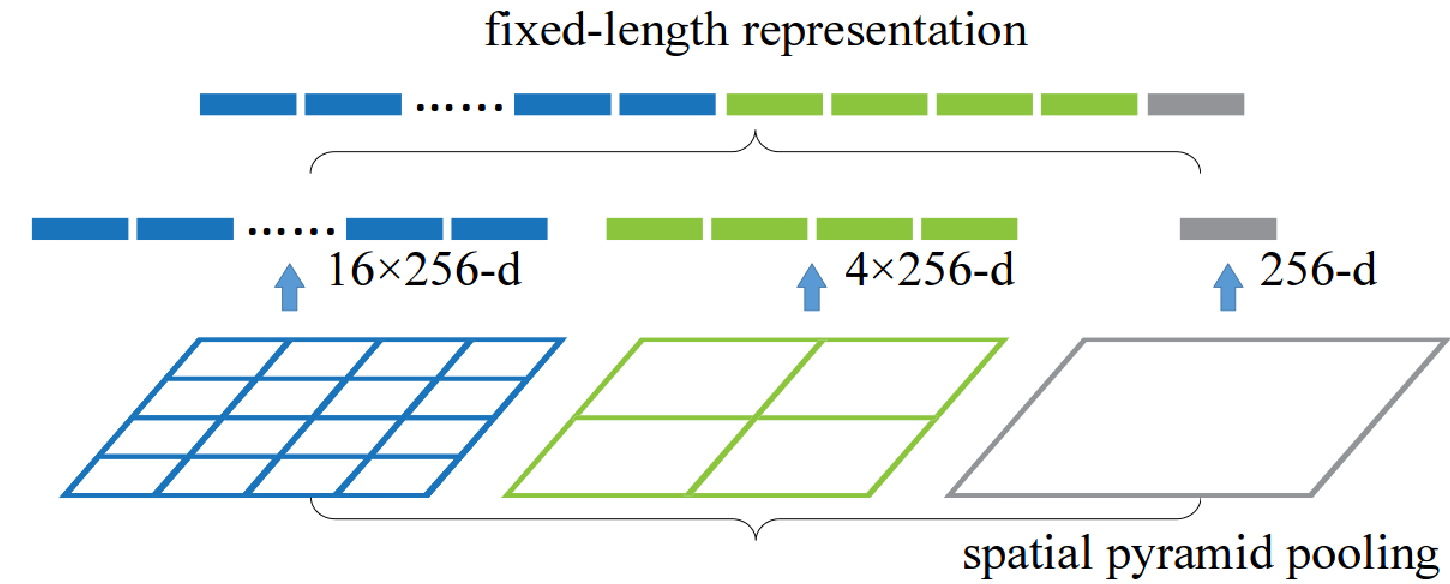
\includegraphics[width=0.8\textwidth]{spp.png}
%\label{fig:spp}
%\caption{Spatial Pyramid Pooling}
%\end{figure}

\subsubsection{Histogram of Oriented Gradients}
Histogram of Oriented Gradients(HOG) are feature descriptors used in computer vision and image processing for the purpose of object detection. The technique counts occurences of gradient orientation in localized portions of an image. HOG descriptors maintains a few advantages over other methods, since it upholds invariance to geometric and photometric transformations, except for object orientation.\par
HOG descriptors are computed using the following steps:
\begin{description}
\item[Gradient Computation] The first step of HOG computes the gradient values, mostly by using the 1-D centered, point discrete derivative mask in one or both of the horizontal and vertical directions.
\item[Orientation Binning] The second step consists of creating the cell histograms. Each pixel within the cell casts a weighted vote for an orientation-based histogram channel based on values found in the gradient computation.
\item[Descriptor Blocks] The third step involves grouping the cells into larger, spatially connected blocks. The HOG descriptor is then the vector of the components of the locally normalized cell histograms from all of the block regions.
\end{description}
In our setting, we scale each image to size $128 \times 128$ and use non-overlapping blocks of size $32 \times 32$, resulting in a 11340 dimensional feature vector. We further trim the feature vector by $75\%$, using $2835$ features each image for training.

\subsubsection{Deep Convolutional Activation Feature}
Recent advances in deep learning have enable researchers to apply deep convolutional neural networks (CNN) to large-scale visual recognition tasks. These models perform extremely well in domains with large amounts of training data, outperforming all known methods on a large scale recognition challenge.\par
However, in other tasks with limited training data, deep neural networks tend to dramatically overfit. To deal with this problem, Donahue et al.(cite) explored a semi-supervised, transfer learning method, which uses a supervised pre-trained deep neural network to extract features. One popular feature selection method is to use activation values in one layer of deep neural network. Donahue et al. have empiracally validated that a generic visual feature based on a convolutional network trained on the ImageNet dataset(cite) outperforms a host of conventional visual representations on standard benchmark object recognition tasks.\par
In our setting, we use the famous AlexNet by Krizhevsky et al. (cite), which contains eight layers with weights: the first five are convolutional and the remaining three are fully connected. The output of the last fully-connected layer is fed to a 1000-way softmax which produces a distribution over the 1000 class labels. The structure of the AlexNet is in figure \ref{fig:alexnet}. Please refer to (cite) for more details of the network. \par

%\begin{figure}
%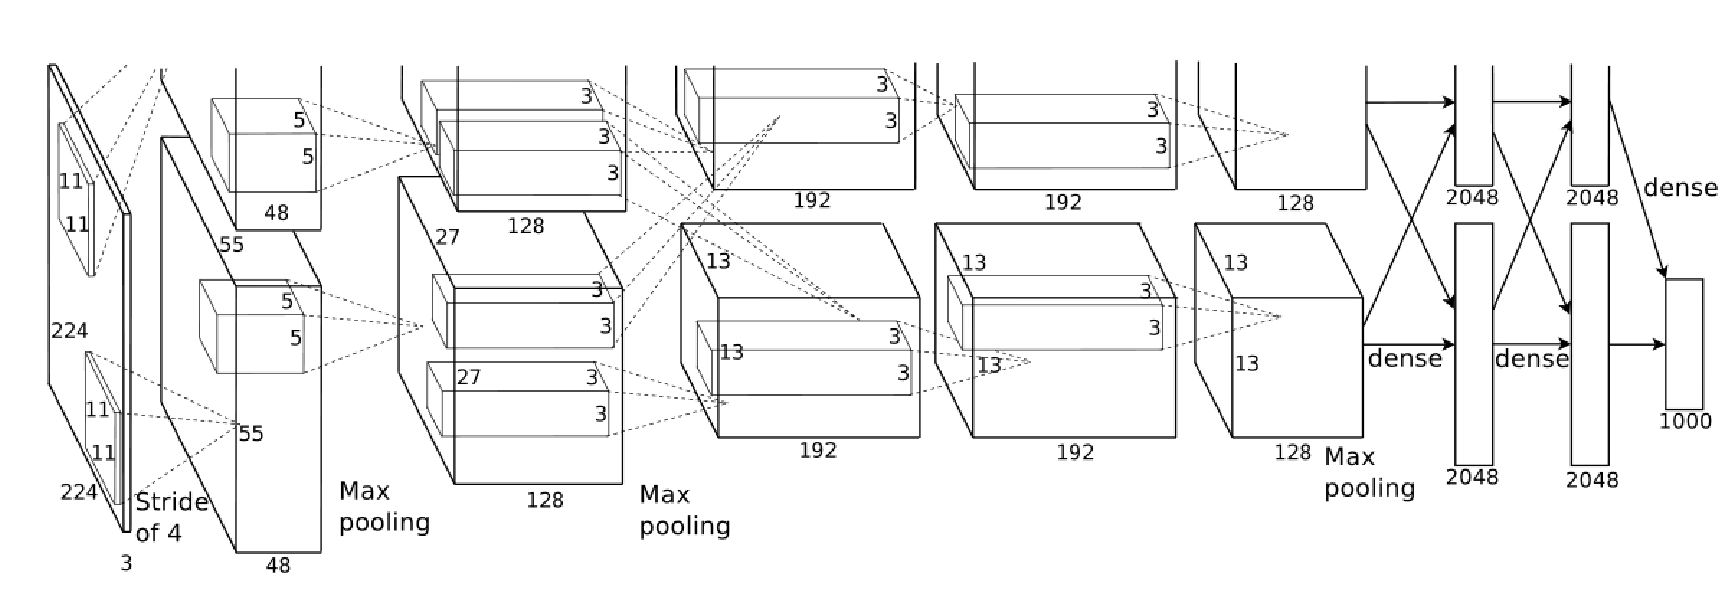
\includegraphics[width=1.0\textwidth]{alexnet.png}
%\label{fig:alexnet}
%\caption{Structure of AlexNet}
%\end{figure}

We use the seventh layer of AlexNet, which has 4096 neuron activations, as our extracted features. We use Caffe(cite), an open source framework for training deep nerual networks on GPUs, and a model trained on ImageNet using Caffe, to extract our features. For each image, we simply do forward propagation, using the image pixel intesities as inputs, and compute the neuron activations of the particular level. Using a GPU, we can speed up the computation by 5 to 10 times.

\subsection{Audio Feature Extraction Techniques}
\subsubsection{Mel-Frequency Cepstrum Coefficients}
In sound processing, the mel-frequency cepstrum is a representation of the short-term power spectrum of a sound, based on a linear cosine transform of a log power spectrum on a non-linear mel scale of frequency. Mel-frequency cepstrum coefficients(MFCCs) are coefficients that collectively make up an MFC, which are derived from a type of cepstral representation of the audio clip. MFCCs are commonly derived as follows:
\begin{enumerate}
\item Take the Fourier transform of a signal
\item Map the powers of the spectrum obtained above onto the mel scale, using triangular overlapping windows.
\item Take the logs of the powers at each of the mel frequencies.
\item Take the discrete cosine transform of the list of mel log powers, as if it were a signal.
\item The MFCs are the amplitudes of the resulting spectrum.
\end{enumerate}
In our setting, we compute the average MFCCs for each shot, so that each shot generates a 12-dimensional feature vector.
\subsubsection{Linear Prediction Coefficients(LPCs)}
Linear prediction is a mathematical opearation where future values of discrete-time signal are estimated as a linear function of previous samples. The most common representation is 
$$ \hat{x}(n) = \sum_{i=1}^{p} a_i x(n-i)$$
where $\hat{x}(n)$ is the predicted signal value, $x(n-i)$ is the previous observed values, and $a_i$ are the predictor coefficients. The error generated by this estimate is 
$$ e(n) = x(n) - \hat{x}(n)$$
where $x(n)$ is the true signal value. \par
The most common choice in optimization of parameters $a_i$ is the root mean square criterion which is also called the auto-correlation criterion. In this method we minimize the L2 norm, which yields the equation:
$$\sum_{i=1}^{p} a_i R(j-i) = -R(j)$$
for $1 \leq j \leq p$, where $R$ is the auto correlation of signal $x_n$, defined as
$$R(i) = \mathrm{E}[x(n)x(n-i)]$$
and $\mathrm{E}$ is the expected value.\par
In our setting, we compute a 12-dimensional feature vector for the LPCs, which gives us a feature vector of length 24 after combining with MFCCs.


\section{Estimation}

\subsection{Dataset}

  The video files in our dataset are collected from CNTV, Youku and Tudou. We manually seperate them into five genres: cartoon, music video(MV), lecture, nature scene, and news report. The total amount of the video information is approximately 1GB. 

  To eliminate the possible negative influence on algorithm performance caused by different video resolution and audio sample rate, these video files are resized and resampled after being downloaded. 

  After processed by ffmpeg, a complete cross-platform solution to record, convert and stream audio and video, the parameters of final video files are listed below.

  \begin{center}
  \begin{tabular}{ccc}
    \hline
    Resolution & frames per second & audio sample rate\\
    480*320 & 15 fps & 44100Hz\\
    \hline
  \end{tabular}
  \end{center}

  To simulate a continue video file for demo system, we concatenate the video segments to a long piece of video. At the same time, the cutting timestamps for different programs are recorded. The timestamps are used to estimate the precision of our system. 

\subsection{Demo Application}

  To estimate the performance of the system, we implement an application for demonstration. This system is developed in C\#, in Microsoft .Net Framework. With windows media player module planted in the application, user can watch the video program by program seemlessly.

  \begin{figure*}
    \centering 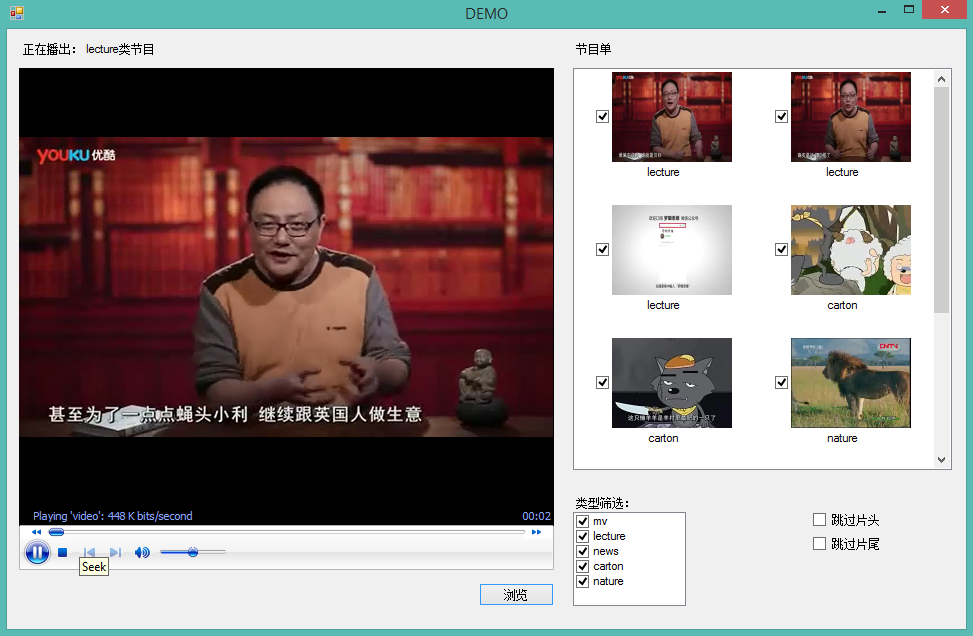
\includegraphics[width=\textwidth]{img/demo.png}
    \caption{The interface of demo application}
  \end{figure*}

  The features of the application are listed below.

  \begin{enumerate}
  \item The application can load from a description file that is the output of our algorithm. The description file contains cutting timestamps for different programs and genre classifications.
  \item The application will fetch one frame as a summery of one program and display the frame as a thumbnail on the interface.
  \item The application can provide a smooth watching experience. There will not be obvious gaps when switching programs. 
  \item Users can filter through different genres of programs. They can choose to watch or not to watch some specific type of programs. Moreover, users can skip a single program without changing other programs with a same genre tag.
  \item The feature of skipping openning and ending scene is on its way.
  \end{enumerate}

\subsection{Experiment}

\subsubsection{audio features}

To calculate LPCs and MFCC features, a python library essentia is used. Essentia is an open-source C++ library for audio analysis and audio-based music information retrieval with Python bindings.

To achieve a better performance, the video clips are segmented into shots firstly. For every single shot of video segment, we calculate the LPCs and MFCC with a window size of 0.02 microsecond and a hop size of 0.01 microsecond. For each slide of time, 12 LPCs and 12 MFCC values will be extracted. After LPCs and MFCC are extracted for a shot, the values will be averaged by time. Thus there will be 12 LPCs and 12 MFCC values for each shot eventually, i.e. 24 audio features for a single shot. 

After audio features extracted, LibSVM is used to estimate the features. The video clips are randomly shaffled into two gruops, the training group and the prediction group. 

Since most of the video clips in the predicition group have a close copy in the training group, the accuracy achieves as high as over 80\%. And both the feature extraction and LibSVM can be done in less than one minute.

The experiment for a larger dataset is on its way.

\subsubsection{combined experiment}

The experiments which combine visual and audio features are on their way.

\section{Future work}

We will focus on combining visual and audio features in the near future. This work will be settled in one week.

Secondly, we plan to come up with a method to combine shots into programs, and run estimations and experiments on shot combining. This may take us two weeks to make it done.

The following table contains more information in detail.

\begin{center}
\begin{tabular}{cc}
  \hline
    Time & Plan
  \hline
    Dec 17, 2014 & Combine visual and audio features
    Dec 20, 2014 & Run estimation for combined features
    Dec 24, 2014 & Concatenate shots into programs
    Dec 27, 2014 & 
  \hline
\end{tabular}
\end{center}

\section{Conclusion}

In this article, we have present our system for video segmentation and classification with a novel way to extract multimedia features and to utilize machine learning methods. We extract SPP, HOG and DNN as visual features, LPC and MFCC as audio features from the original video file. We combine the features and then classify the video into five genres. We use the classification information to gather shots into programs. We implement an application that can parse the result of our algorithm, and playback the video with these additional information.

With detailed experiments and estimation, we have proved that our algorithm is able to classify the genres of video segments with great precision and efficience. We have compared our algorithm with traditional methods and proved that our method overwhelm traditional methods in both speed and precision. 

There are still a lot more space for us to improve our performance. 1) Because of the limit of the size of dataset, our machine learning model is not fully trained. Thus with more labeled video data which covers more cases, we confidently believe that our model can have a better performance. 2) We hope we can come up with a way to improve our model accumulatively, which is to train our model each time a new video comes, instead of once-trained-use-forever model.

\bibliography{a}
\bibliographystyle{icml2014}

\end{document} 


% This document was modified from the file originally made available by
% Pat Langley and Andrea Danyluk for ICML-2K. This version was
% created by Lise Getoor and Tobias Scheffer, it was slightly modified  
% from the 2010 version by Thorsten Joachims & Johannes Fuernkranz, 
% slightly modified from the 2009 version by Kiri Wagstaff and 
% Sam Roweis's 2008 version, which is slightly modified from 
% Prasad Tadepalli's 2007 version which is a lightly 
% changed version of the previous year's version by Andrew Moore, 
% which was in turn edited from those of Kristian Kersting and 
% Codrina Lauth. Alex Smola contributed to the algorithmic style files.  
